\documentclass[conference]{IEEEtran}

\usepackage{cite}
% \usepackage[hidelinks]{hyperref}
\usepackage{hyperref}
\usepackage{graphicx}
\usepackage{subcaption}
\usepackage{array}
\usepackage{booktabs}

\hyphenation{op-tical net-works semi-conduc-tor}


\begin{document}
%
% paper title
% Titles are generally capitalized except for words such as a, an, and, as,
% at, but, by, for, in, nor, of, on, or, the, to and up, which are usually
% not capitalized unless they are the first or last word of the title.
% Linebreaks \\ can be used within to get better formatting as desired.
% Do not put math or special symbols in the title.
\title{Advancements, Challenges, and Future Prospects in\\ Agricultural Remote Sensing: A Review}


% author names and affiliations
% use a multiple column layout for up to three different
% affiliations
\author{\IEEEauthorblockN{Xiaotong Zhou}
\IEEEauthorblockA{School of Computer Science\\
Nanjing University of Information Science \& Technology\\
Nan Jing, Jiang Su, China, 210031\\
Email: zxt1428147954@163.com}
}
% conference papers do not typically use \thanks and this command
% is locked out in conference mode. If really needed, such as for
% the acknowledgment of grants, issue a \IEEEoverridecommandlockouts
% after \documentclass

% for over three affiliations, or if they all won't fit within the width
% of the page, use this alternative format:
% 
%\author{\IEEEauthorblockN{Michael Shell\IEEEauthorrefmark{1},
%Homer Simpson\IEEEauthorrefmark{2},
%James Kirk\IEEEauthorrefmark{3}, 
%Montgomery Scott\IEEEauthorrefmark{3} and
%Eldon Tyrell\IEEEauthorrefmark{4}}
%\IEEEauthorblockA{\IEEEauthorrefmark{1}School of Electrical and Computer Engineering\\
%Georgia Institute of Technology,
%Atlanta, Georgia 30332--0250\\ Email: see http://www.michaelshell.org/contact.html}
%\IEEEauthorblockA{\IEEEauthorrefmark{2}Twentieth Century Fox, Springfield, USA\\
%Email: homer@thesimpsons.com}
%\IEEEauthorblockA{\IEEEauthorrefmark{3}Starfleet Academy, San Francisco, California 96678-2391\\
%Telephone: (800) 555--1212, Fax: (888) 555--1212}
%\IEEEauthorblockA{\IEEEauthorrefmark{4}Tyrell Inc., 123 Replicant Street, Los Angeles, California 90210--4321}}




% use for special paper notices
%\IEEEspecialpapernotice{(Invited Paper)}




% make the title area
\maketitle

% As a general rule, do not put math, special symbols or citations
% in the abstract
\begin{abstract}
  Agricultural remote sensing, a crucial component of precision agriculture, leverages advanced technologies to monitor and manage crop production efficiently. This report delves into the applications, challenges, and future prospects of agricultural remote sensing. It highlights the significant role of high-resolution data and intelligent analysis in real-time agricultural monitoring and decision-making. The report also addresses the challenges in technology adoption and proposes solutions such as enhanced training and user-friendly tools. Finally, it explores the future trends of integrating deep learning and IoT with remote sensing for intelligent agricultural management.
\end{abstract}

% no keywords




% For peer review papers, you can put extra information on the cover
% page as needed:
% \ifCLASSOPTIONpeerreview
% \begin{center} \bfseries EDICS Category: 3-BBND \end{center}
% \fi
%
% For peerreview papers, this IEEEtran command inserts a page break and
% creates the second title. It will be ignored for other modes.
\IEEEpeerreviewmaketitle


\section{Introduction}

In recent years, the agricultural sector has witnessed significant technological advancements, with remote sensing emerging as a pivotal tool for modern farming practices. Agricultural remote sensing involves the use of satellite imagery, aerial photography, and ground-based sensors to collect data on various aspects of crop production\cite{bastiaanssenRemoteSensingIrrigated2000}\cite{geRemoteSensingSoil2011}\cite{huangAgriculturalRemoteSensing2018}\cite{javedPerformanceRelationshipFour2021}. This technology enables farmers and agronomists to monitor crop health, soil conditions, and environmental factors with unprecedented precision and efficiency.

The integration of remote sensing into agriculture offers numerous benefits, including improved crop management, optimized resource use, and enhanced decision-making capabilities\cite{javedPerformanceRelationshipFour2021}. By providing detailed, real-time information, remote sensing helps farmers make informed decisions about irrigation, fertilization, pest control, and harvesting. This not only increases crop yields but also promotes sustainable farming practices by reducing the unnecessary use of inputs and minimizing environmental impacts.

However, the application of remote sensing in agriculture is not without its challenges\cite{ozdoganRemoteSensingIrrigated2010}. Issues such as data acquisition and processing, model complexity, and the acceptance of technology by farmers pose significant barriers to its widespread adoption. Addressing these challenges requires a multifaceted approach, including the development of advanced analytical methods, user-friendly tools, and effective training programs.

This report explores the current state of agricultural remote sensing, focusing on the challenges and solutions associated with its implementation. It also examines future trends and research directions that have the potential to further enhance the capabilities and applications of this transformative technology.


\section{Background}

\subsection{Background of Remote Sensing}

Since the development of remote sensing technology in the early 20th century, it has undergone significant technological advancements and application expansions. The earliest applications of remote sensing technology can be traced back to photogrammetry techniques using balloons and airplanes\cite{bastiaanssenRemoteSensingIrrigated2000}. After World War II, with the advancement of space technology, satellite remote sensing gradually became mainstream. In 1972, the United States launched the first Earth Resources Technology Satellite (Landsat-1), marking the beginning of the modern satellite remote sensing era. Subsequently, various countries launched multiple remote sensing satellites, such as France's SPOT series\cite{SPOTsate81:online}, Japan's ALOS series\cite{Advanced84:online}, and Europe's Sentinel series\cite{Sentinel88:online}. These satellites have greatly enhanced the capability to acquire and apply remote sensing data.

\begin{figure}[htbp!]
    \centering
    \begin{subfigure}[b]{0.15\textwidth}
        \centering
        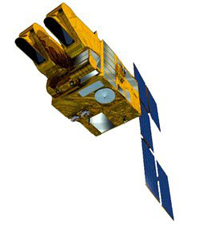
\includegraphics[height=0.1\textheight]{figs/Spot-5.jpg}
        \caption{SPOT}
    \end{subfigure}
    \begin{subfigure}[b]{0.15\textwidth}
        \centering
        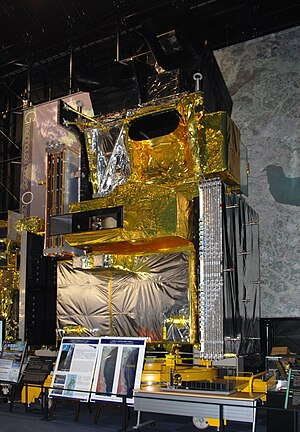
\includegraphics[height=0.1\textheight]{figs/AlOS.jpg}
        \caption{ALOS}
    \end{subfigure}
    \begin{subfigure}[b]{0.15\textwidth}
        \centering
        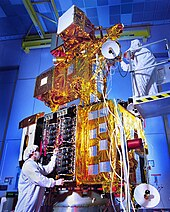
\includegraphics[height=0.1\textheight]{figs/Landsat7photo.jpg}
        \caption{Landsat}
    \end{subfigure}
    \caption{Several Satellites}
\end{figure}
Currently, remote sensing technology is widely used in various fields such as environmental monitoring\cite{li2020review}, urban planning\cite{wellmann2020remote}, resource management\cite{kumar2015applications}, and disaster warning\cite{gupta2022smart}. With continuous technological advancements, the spatial resolution, spectral resolution, and temporal resolution of remote sensing data have significantly improved. In particular, the development of hyperspectral remote sensing and Synthetic Aperture Radar (SAR)\cite{Syntheti6:online} technology has further expanded the precision and scope of remote sensing applications.

\subsection{Development and Application of Big Data}

The rapid development of big data technology has had a profound impact on various fields. Big data typically refers to data sets that cannot be processed using traditional database tools and are characterized by their large volume, variety of data types, high velocity of processing, and high value. Big data technology encompasses multiple stages, including data collection, storage, processing, analysis, and visualization, involving distributed computing frameworks like Hadoop and Spark, as well as data analysis methods such as machine learning and data miningc\cite{mandalImpactAgriculturalManagement2022}.

In the agricultural sector, the application of big data technology includes the collection and analysis of agricultural production data, monitoring and prediction of meteorological data, and analysis and forecasting of market information. Through comprehensive analysis of these data, scientific decision support can be provided for agricultural production, improving production efficiency and reducing resource waste and environmental pollution.

\subsection{Definition and Development of Agricultural Remote Sensing}

Agricultural remote sensing refers to the use of remote sensing technology to acquire and analyze various information in agricultural production to support scientific decision-making in agriculture. The development of agricultural remote sensing can be traced back to the 1960s, when aerial photography technology was primarily used to monitor farmland. With the advancement of satellite remote sensing technology, the application scope and accuracy of agricultural remote sensing have greatly improved.

Modern agricultural remote sensing technology utilizes various platforms, including satellites, drones, and ground sensors, to acquire high-resolution remote sensing data\cite{mullaTwentyFiveYears2013}. By analyzing this data, real-time monitoring of crop growth, pest and disease occurrences, soil moisture, and fertility can be achieved. Agricultural remote sensing technology not only improves agricultural production efficiency but also reduces the use of pesticides and fertilizers, thereby decreasing environmental pollution.

\subsection{The Importance of Agricultural Remote Sensing in Modern Agriculture}

Agricultural remote sensing holds significant application value in modern agriculture. Firstly, it enables real-time monitoring and management of large-scale farmland. Traditional agricultural production management methods often rely on manual surveys and experiential judgments, which are inefficient, costly, and not highly accurate. Remote sensing technology allows for the rapid acquisition of high-precision data over vast areas of farmland, enabling refined management of the fields.

Secondly, agricultural remote sensing technology can improve crop yield and quality. By monitoring crop growth conditions in real time, issues can be promptly identified, and appropriate measures can be taken to prevent the impact of pests, diseases, and adverse environmental factors on crops\cite{kasampalisContributionRemoteSensing2018}. Additionally, remote sensing technology can be used for crop yield prediction, providing a scientific basis for agricultural production.

Lastly, agricultural remote sensing technology plays an important role in environmental protection. Through remote sensing technology, the usage of soil and water resources can be monitored, the impact of agricultural production on the environment can be assessed, and scientific resource management and environmental protection strategies can be formulated.
\section{Overview of Remote Sensing}

\subsection{Basic Principles of Agricultural Remote Sensing}

\subsubsection{Basic Principles of Remote Sensing Technology}

Remote sensing technology is a method of obtaining and analyzing information about target objects and their environments from a distance. It primarily relies on sensors to receive electromagnetic waves reflected or emitted by target objects, which are then processed and analyzed to extract useful information. The basic principles of remote sensing technology can be summarized in the following steps\cite{geRemoteSensingSoil2011}:

\paragraph{Energy Source or Illumination} The remote sensing process typically depends on solar energy or artificial electromagnetic sources (such as radar). Sunlight, as a natural energy source, is reflected or absorbed by surface objects and re-emitted at different wavelengths.

\paragraph{Interaction between Energy and Target}Different objects have unique reflection, absorption, and emission characteristics for different wavelengths of electromagnetic waves, known as spectral characteristics. Plants, water bodies, and soil exhibit different spectral reflectance in various bands, forming the basis for remote sensing identification and classification.

\paragraph{Sensor Reception of Energy}Sensors mounted on satellites, aircraft, or drones receive electromagnetic waves reflected or emitted by target objects. Depending on their operational wavelength bands, sensors can be categorized into visible light sensors, infrared sensors, microwave sensors, and more.

\paragraph{Data Transmission and Processing} Electromagnetic signals received by sensors are converted and encoded, then transmitted to ground receiving stations via radio waves. These signals undergo preprocessing (such as atmospheric correction, geometric correction, radiometric correction) to generate remote sensing image data for analysis.

\paragraph{Data Analysis and Application} Processed remote sensing data are further analyzed to extract information on spatial distribution, spectral characteristics, and temporal changes of target objects, applicable in fields such as agriculture, environmental monitoring, and urban planning.

\subsubsection{Optical Remote Sensing Technology in Agriculture}

Optical remote sensing technology, widely used in agricultural remote sensing, primarily utilizes electromagnetic waves in the visible and near-infrared bands for observation. The basic principle is to receive sunlight reflected by surface objects through sensors and analyze the spectral reflectance in different bands to identify and monitor land cover.

\paragraph{Spectral Reflectance Characteristics} Plants, soil, and water bodies exhibit different spectral reflectance characteristics in the visible and near-infrared bands. For example, healthy plants have high reflectance in the near-infrared band (700-1300 nm) and low reflectance in the red band (600-700 nm). Analyzing these spectral characteristics can assess plant health, identify crop types, and monitor soil moisture.

\paragraph{Typical Optical Remote Sensing Indices} Common optical remote sensing indices include the Normalized Difference Vegetation Index (NDVI)\cite{Normaliz41:online} and the Enhanced Vegetation Index (EVI)\cite{Enhanced85:online}. NDVI\cite{Normaliz41:online}, an index measuring vegetation cover and health, is calculated as follows:

\begin{equation}
        \textbf{NVDI} = \frac{\textbf{NIR}-\textbf{Red}}{\textbf{NIR}+\textbf{Red}}
        \label{formula:NVDI}
\end{equation}

where NIR represents the reflectance in the near-infrared band, and Red represents the reflectance in the red band. NDVI values range from -1 to 1, with positive values indicating vegetation cover, and higher values indicating healthier vegetation.

\paragraph{Applications of Optical Remote Sensing} Optical remote sensing is widely applied in crop monitoring, soil analysis, and pest identification. For example, by periodically acquiring optical remote sensing images, crop growth changes can be monitored to timely identify and address issues in agricultural production.

\subsubsection{Radar Remote Sensing Technology in Agriculture}

Radar remote sensing technology utilizes electromagnetic waves in the microwave band (1 mm - 1 m) for observation, capable of all-weather, day-and-night operation. The basic principle involves sensors emitting microwave signals and receiving signals reflected by surface objects, analyzing reflection characteristics and phase information.

\paragraph{Synthetic Aperture Radar (SAR)} SAR, a commonly used radar remote sensing technology, enhances resolution by synthesizing a large aperture antenna. SAR sensors can operate under adverse weather conditions (e.g., cloud cover, rainfall), making them crucial for agricultural remote sensing.

\paragraph{Reflection Characteristics of Radar Signals} Different surface objects have unique reflection characteristics for microwave signals. For example, moist soil and vegetation reflect microwave signals more strongly than dry soil. By analyzing the intensity and phase information of radar images, structural, moisture, and topographical information of surface objects can be obtained.

\paragraph{Applications of Radar Remote Sensing} Radar remote sensing technology is important for soil moisture monitoring, crop growth monitoring, and disaster assessment. For instance, analyzing SAR images from different time points can monitor changes in farmland soil moisture, providing a basis for precision irrigation.

\subsubsection{Thermal Infrared Remote Sensing Technology in Agriculture}

Thermal infrared remote sensing technology utilizes electromagnetic waves in the thermal infrared band (8-14 µm) to measure surface temperature. The basic principle involves sensors receiving thermal infrared radiation emitted by surface objects and analyzing temperature distribution characteristics.

\paragraph{Thermal Infrared Radiation Characteristics} Different surface objects have unique radiation characteristics in the thermal infrared band. For example, vegetation has low thermal radiation intensity at night, while bare soil and buildings have higher thermal radiation intensity. Analyzing the radiation intensity in thermal infrared images can estimate surface temperature and identify different objects.

\paragraph{Applications of Thermal Infrared Remote Sensing} Thermal infrared remote sensing technology is crucial for monitoring crop water stress, irrigation management, and pest warning. For instance, monitoring temperature changes in farmland can assess whether crops are experiencing water stress, guiding precision irrigation.

In summary, agricultural remote sensing technology utilizes electromagnetic waves in optical, radar, and thermal infrared bands to achieve real-time monitoring and management of farmland. Optical remote sensing is suitable for monitoring vegetation health and crop classification, radar remote sensing is ideal for soil moisture monitoring and disaster assessment, and thermal infrared remote sensing is effective for surface temperature measurement and irrigation management. The comprehensive application of these technologies provides robust technical support for precision agriculture and sustainable agricultural development.
\subsection{Acquisition of Agricultural Remote Sensing Data}

\subsubsection{Data Acquisition Platforms}
The acquisition of agricultural remote sensing data primarily relies on three platforms: satellite remote sensing, UAV\cite{Unmanned27:online} remote sensing, and ground sensors\cite{mandalImpactAgriculturalManagement2022}. Each of these platforms has its own advantages and disadvantages, catering to different application needs.

\begin{figure}[htbp!]
    \centering
    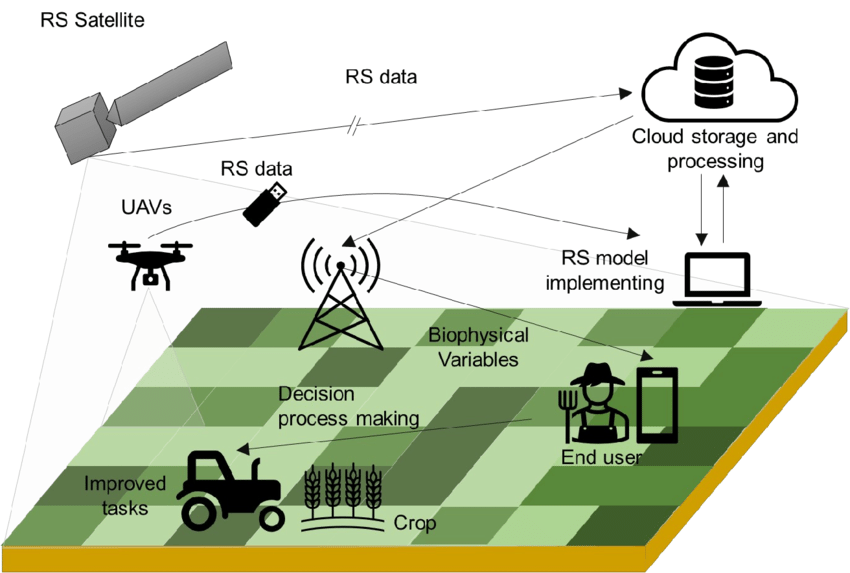
\includegraphics[width=0.35\textwidth]{figs/remote_sensing.png}
    \caption{Remote Sensing and Agricultural}
\end{figure}

\paragraph{Satellite Remote Sensing}

Satellite remote sensing is the most commonly used method for acquiring agricultural remote sensing data. Remote sensors mounted on satellites orbiting the Earth can regularly and continuously obtain large-scale surface information.

Satellite remote sensing has many advantages. Satellite remote sensing can cover global areas, suitable for monitoring large-scale farmland. Most remote sensing satellites can regularly obtain data, suitable for long-term monitoring of crop growth dynamics. Many satellites are equipped with multispectral sensors that can obtain data in various bands such as visible light, near-infrared, and shortwave infrared, suitable for various agricultural applications\cite{sahooHyperspectralRemoteSensing2015}.


Here are some application cases about this kind of sensors.

Landsat Series\cite{Landsatp77:online}: Jointly launched by the U.S. Geological Survey (USGS) and NASA, the Landsat series satellites provide medium-resolution multispectral data widely used in land use and crop monitoring.

Sentinel Series\cite{Sentinel88:online}: The European Space Agency (ESA)'s Sentinel series satellites include both multispectral and radar remote sensing data, suitable for agriculture, environmental monitoring, and other applications.

MODIS\cite{MODISWeb11:online}: The MODIS sensors on NASA's Terra and Aqua satellites provide high temporal resolution, medium-to-low resolution data suitable for large-scale agricultural monitoring.

%『插入图像:对应的卫星图像』

\paragraph{UAV Remote Sensing}

UAV (unmanned aerial vehicle)\cite{Unmanned27:online}(Fig.\ref{fig:UAVs}) remote sensing is a highly flexible data acquisition method. UAVs equipped with high-resolution sensors can fly at low altitudes to obtain high-precision surface information.

As they fly at low altitudes, UAVs\cite{Unmanned27:online} can capture high-resolution images suitable for detailed farmland monitoring. Moreover, UAV\cite{Unmanned27:online} flight plans can be flexibly adjusted according to needs, adapting to different task requirements. Compared to satellite remote sensing, UAV\cite{Unmanned27:online} remote sensing is less costly, suitable for small-scale agricultural applications.

Here are some application cases about this kind of sensors.

Crop Health Monitoring\cite{javedPerformanceRelationshipFour2021}: By acquiring high-resolution multispectral and thermal infrared images, UAVs\cite{Unmanned27:online} can monitor the growth and health of crops, identifying pests and nutrient deficiencies early.

Precise Farmland Management: UAV\cite{Unmanned27:online} remote sensing data can be used for precise farmland management, such as targeted fertilization and irrigation, optimizing the use of agricultural resources.

\begin{figure*}[htbp!]
    \centering
    \begin{subfigure}[b]{0.3\textwidth}
        \centering
        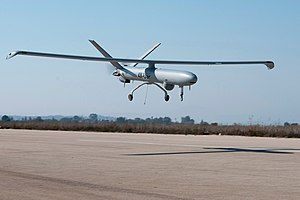
\includegraphics[height=0.15\textheight]{figs/U1.jpg}
        \caption{Elbit Systems Hermes-450}
    \end{subfigure}
    \begin{subfigure}[b]{0.3\textwidth}
        \centering
        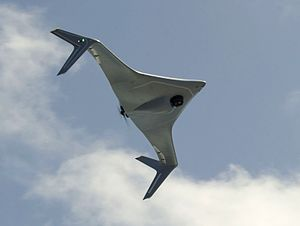
\includegraphics[height=0.15\textheight]{figs/U2.jpg}
        \caption{Northrop Grumman Bat}
    \end{subfigure}
    \begin{subfigure}[b]{0.3\textwidth}
        \centering
        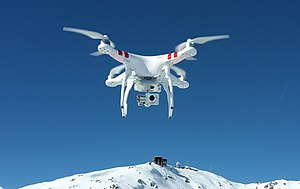
\includegraphics[height=0.15\textheight]{figs/U3.jpg}
        \caption{DJI Phantom quadcopter UAV}
    \end{subfigure}
    \caption{UAVs (Unmanned Aerial Vehicles)}
    \label{fig:UAVs}
\end{figure*}

\paragraph{Ground Sensors}

Ground sensors are devices installed on the ground to monitor various environmental parameters of farmland in real-time. Common ground sensors include soil moisture sensors, weather stations, and chlorophyll sensors.

Different from satellite remote sensing, ground sensors can collect data in real-time, which are suitable for dynamic monitoring\cite{khanalRemoteSensingAgriculture2020}. Ground sensors can also obtain high-precision environmental parameters such as soil moisture and temperature. Many ground sensors directly contact the target object, providing highly reliable data.

Here are some application cases about this kind of sensors.

Soil Moisture Monitoring: Soil moisture sensors can monitor the water content of farmland soil in real-time, providing data support for precision irrigation.

Meteorological Monitoring: Weather stations can monitor meteorological parameters such as temperature, precipitation, and wind speed, providing weather forecasts and risk assessments for agricultural production.

\subsubsection{Spatiotemporal Resolution Requirements for Data Acquisition}

The spatiotemporal resolution requirements of agricultural remote sensing data depend on specific application needs. Spatiotemporal resolution refers to the spatial and temporal resolution of remote sensing data.

\paragraph{Spatial Resolution}

Spatial resolution refers to the smallest size of the surface object that the sensor can distinguish. High spatial resolution data can provide more detailed surface information, suitable for precise farmland management; low spatial resolution data are suitable for large-scale regional monitoring.
Crop classification requires medium to high spatial resolution (10-30 meters) data to accurately identify different types of crops. Pest monitoring requires high spatial resolution (<10 meters) data to detect and locate pest-infested areas early. Soil moisture monitoring generally requires medium to low spatial resolution (>30 meters) data, which can usually meet the needs.

\paragraph{Temporal Resolution}

Temporal resolution refers to the frequency at which the sensor acquires data. High temporal resolution data can provide continuous time series information, suitable for dynamic monitoring; low temporal resolution data are suitable for monitoring changes over long time scales.
Crop growth monitoring requires high temporal resolution (daily or weekly) data to detect and address issues arising during the growth process promptly.
Agricultural disaster (e.g., drought, flood) monitoring requires high temporal resolution data to quickly assess the impact of the disaster and develop response measures.
Long-term change monitoring of land use and climate change impacts on agricultural production can use low temporal resolution (monthly or yearly) data.

In conclusion, the acquisition of agricultural remote sensing data relies on satellite remote sensing, UAV remote sensing, and ground sensors, each with its unique advantages and applicable scope. Choosing appropriate spatiotemporal resolutions according to specific application needs can effectively enhance the application effectiveness of remote sensing data. By comprehensively utilizing data from different platforms and resolutions, it is possible to achieve comprehensive, detailed, and dynamic monitoring and management of farmland, providing strong technical support for precision agriculture and sustainable agricultural development.

\section{Processing and Analysis of Data}

\subsection{Data Preprocessing}
Data preprocessing is a crucial step in agricultural remote sensing data analysis, involving data correction and data fusion. Data correction ensures the accuracy and consistency of remote sensing data, while data fusion integrates multi-source data to enhance the spatial, temporal, and spectral resolution, providing richer information for subsequent analysis.

Data Correction\cite{huangAgriculturalRemoteSensing2018}.
Data correction involves processing raw remote sensing data to eliminate various errors, ensuring data authenticity and accuracy. Common types of data correction include atmospheric correction, geometric correction, and radiometric correction.

Atmospheric Correction\cite{seelanRemoteSensingApplications2003}. 
Atmospheric correction involves eliminating the effects of the atmosphere on remote sensing data. Due to the scattering and absorption by atmospheric molecules and aerosols, the electromagnetic signals received by remote sensing sensors are distorted and attenuated. Therefore, atmospheric correction is a key step in accurately restoring surface reflectance. Here are some methods to do this task.
Absolute Correction Method: Based on atmospheric radiation transfer models (such as MODTRAN and 6S), correction is performed by retrieving atmospheric parameters (such as water vapor content and aerosol optical thickness).
Relative Correction Method: Utilizing ground truth data or concurrent multispectral images for relative correction, such as the radiometric normalization method and dark object subtraction method.

Geometric Correction\cite{geRemoteSensingSoil2011}.
Geometric correction maps remote sensing images to a geographic coordinate system, eliminating geometric distortions caused by sensor attitude, terrain relief, and Earth's curvature. Here are some methods to do this task.Geometric Precision Correction: Utilizing ground control points (GCP) and high-precision digital elevation models (DEM), correction is achieved through polynomial transformation or rigorous orthorectification. Orthorectification: Using DEM to eliminate terrain-induced image distortions, aligning images with their true ground positions.

Radiometric Correction\cite{ulloAdvancesIoTSmart2021}.
Radiometric correction converts raw image DN values into actual surface reflectance or radiance values, eliminating the influence of sensor performance and observation conditions on radiometric values.Here are some methods to do this task.
Absolute Radiometric Correction: Using sensor calibration parameters and solar irradiance for correction to calculate surface reflectance.
Relative Radiometric Correction: Using multi-temporal images for relative correction to maintain radiometric consistency between images, such as the radiometric normalization method.

Data Fusion.
Data fusion integrates multi-source remote sensing data to enhance overall data performance. Data fusion can be categorized into spatial fusion, temporal fusion, and spectral fusion.

Spatial Fusion\cite{weissRemoteSensingAgricultural2020}.
Spatial fusion combines low spatial resolution data with high spatial resolution data to generate data with both high spatial and high spectral resolution. Here are some methods to do this task.
Principal Component Analysis (PCA): Utilizing principal component analysis, the principal components of high-resolution images are merged with low-resolution multispectral images.
Brovey Transform: Calculating the ratio of each band and merging high-resolution images with low-resolution multispectral images.
Wavelet Transform: Using wavelet transform to merge detailed information from high-resolution images with low-resolution multispectral images.

Temporal Fusion.
Temporal fusion merges remote sensing data acquired at different times to generate data with high temporal resolution, suitable for dynamic monitoring. Here are some methods to do this task\cite{huangAgriculturalRemoteSensing2018}.
Time Series Interpolation Method: Using time series interpolation algorithms (such as linear interpolation and spline interpolation) to merge images from different times, creating continuous time series data.
Data Assimilation Method: Employing data assimilation techniques to merge remote sensing observations with numerical models to improve temporal resolution.

Spectral Fusion.
Spectral fusion merges data with different spectral resolutions to generate data with high spectral resolution, enhancing spectral information richness.
Hyperspectral and Multispectral Fusion: Combining spectral information from hyperspectral images with spatial information from multispectral images, such as the hyperspectral decomposition method.
Multi-band Fusion: Merging multi-band data from different sensors to generate images with rich spectral information. 

Data preprocessing is a crucial step in agricultural remote sensing data analysis, ensuring data accuracy and consistency. Atmospheric correction, geometric correction, and radiometric correction eliminate various errors, enhancing data quality. Data fusion techniques integrate multi-source data to improve spatial, temporal, and spectral resolution, providing a solid data foundation for various agricultural remote sensing applications. By comprehensively utilizing data correction and data fusion techniques, it is possible to achieve fine, dynamic, and comprehensive monitoring of farmland, providing strong technical support for precision agriculture and sustainable agricultural development.
\subsection{Feature Extraction}

Feature extraction is a critical step in agricultural remote sensing data analysis. By extracting useful spectral and temporal features, it is possible to identify and monitor crop growth status, health conditions, and environmental changes\cite{mullaTwentyFiveYears2013}. The methods for feature extraction include spectral feature extraction and time series analysis.

\subsubsection{Spectral Feature Extraction}

Spectral feature extraction involves deriving indicators that reflect the characteristics of ground objects from the spectral data of remote sensing images. Common spectral features include the Normalized Difference Vegetation Index (NDVI) and the Enhanced Vegetation Index (EVI).

\paragraph{Normalized Difference Vegetation Index (NDVI)}

NDVI is a spectral index that measures vegetation cover and health status. Its calculation formula is introduced before at Formula. \ref{formula:NVDI}.

Here are some applications.
Crop Health Monitoring: Analyzing NDVI values can assess crop health and vigor.
Land Cover Classification: NDVI can differentiate between vegetation, bare land, and water bodies.
Drought Monitoring: Changes in NDVI values can reflect vegetation water stress, making it suitable for drought monitoring.

\paragraph{Enhanced Vegetation Index (EVI)}

EVI\cite{Enhanced25:online} is a vegetation index developed from NDVI that reduces the influence of atmospheric and soil background effects. Its calculation formula is:

\begin{equation}
    \textbf{EVI} = G \times \frac{NIR - Red}{NIR + C_1 \times Red - C_2 \times Blue + L}
\end{equation}

where NIR, Red, and Blue are the reflectance values in the near-infrared, red, and blue bands respectively. G is a gain factor (usually 2.5), C1 and C2 are correction coefficients (usually 6 and 7.5), and L is an adjustment factor (usually 1)\cite{khanalRemoteSensingAgriculture2020}.

Here are some applications.
High-Density Vegetation Monitoring: EVI performs better than NDVI in areas with dense vegetation, making it suitable for monitoring dense forests and crops.
Crop Growth Analysis: EVI can be used to assess crop vigor and growth changes.

\subsubsection{Time Series Analysis}

Time series analysis uses multi-temporal remote sensing data to analyze the temporal variation characteristics of target objects. By performing time series analysis, it is possible to dynamically monitor crop growth processes and evaluate changes and trends in agricultural production.

\subsubsection{Crop Growth Monitoring}

Crop growth monitoring involves analyzing spectral and morphological features of crops at different times to assess their growth status and trends. Common time series analysis methods include time series models, trend analysis, and change detection.

Several methods are applied to this kind of monitoring.
Time Series Models: Using time series models (such as autoregressive models and ARIMA models) to analyze changes and trends in crop growth, predicting future growth.
Trend Analysis: Evaluating crop growth dynamics and health status by calculating the trend of spectral indices (such as NDVI and EVI) from multi-temporal data.
Change Detection: Identifying abnormal changes in crop growth processes using change detection algorithms (such as image differencing and principal component analysis), such as pest outbreaks and water stress.

Here are some applications.
Crop Growth Monitoring: Evaluating crop growth dynamics and vigor by analyzing changes in NDVI or EVI values from multi-temporal data.
Farm Management: Time series analysis helps farmers timely detect and address issues in crop growth, optimizing agricultural management practices.
Disaster Early Warning: Monitoring temporal changes in crops can provide early warnings of agricultural disasters like droughts and floods, reducing disaster losses.
\subsection{Data Analysis and Model Construction}

In the field of agricultural remote sensing, data analysis and model construction are critical steps for tasks such as crop monitoring, classification, and pest identification. In recent years, the application of machine learning and deep learning technologies in agricultural remote sensing has made significant progress, providing robust technical support for precision agriculture. This section will comprehensively introduce the applications of machine learning and deep learning in agricultural remote sensing, including supervised learning, unsupervised learning, and the use of Convolutional Neural Networks (CNN).

\subsubsection{Applications of Machine Learning in Agricultural Remote Sensing}

Machine learning techniques are widely applied in agricultural remote sensing. They encompass supervised and unsupervised learning methods, each suitable for various application scenarios and data characteristics\cite{weissRemoteSensingAgricultural2020}. Supervised learning utilizes labeled data for training to establish mapping relationships between input data and output labels. Common supervised learning algorithms include Support Vector Machines (SVM), Random Forests (RF), Gradient Boosting Decision Trees (GBDT), among others. These algorithms enable accurate classification of different crop types (e.g., corn, wheat, rice) using multispectral remote sensing data. They can also identify regions affected by pests and diseases on crop leaves, leveraging GBDT models for disease spot detection and pest type identification.

Supervised learning offers high accuracy by leveraging labeled data for training. It provides flexibility in choosing algorithms and features based on specific requirements. 

Nonetheless, unsupervised learning analyzes and clusters data based on internal structures and distribution patterns, bypassing the need for labeled data. K-means clustering, Principal Component Analysis (PCA), and other algorithms facilitate automatic classification of land surfaces based on remote sensing image spectral characteristics. Furthermore, they detect abnormal changes in remote sensing data, such as disease outbreaks or droughts, using PCA algorithms to detect crop growth anomalies.

Unsupervised learning benefits from not requiring extensive labeled data and is applicable in scenarios where labeling is challenging despite large datasets. It allows the automatic discovery of patterns and structures within the data.

\subsubsection{Deep Learning Models}

Deep learning is a prominent branch of machine learning that has achieved remarkable success in image processing and analysis. Convolutional Neural Networks (CNNs) are classic models within deep learning widely used in image classification and object detection tasks.

Convolutional Neural Networks (CNNs) process image data with specialized neural network structures, automatically extracting image features through convolutional layers, pooling layers, and fully connected layers. CNN models utilize multispectral or hyperspectral data to classify various crop types accurately, employing architectures like LeNet, AlexNet, VGG, ResNet, among others.

CNNs achieve high precision in classification tasks by automatically extracting high-order features from images. They support end-to-end learning from raw data to classification results, reducing feature engineering complexity.

Additionally, CNNs' convolutional layers extract local features from images, while fully connected layers integrate these features for complex pattern recognition. By training CNN models with high-resolution images, automatic identification and classification of various pests and diseases on crop leaves can be achieved. CNN architectures such as Inception, DenseNet, MobileNet, among others, enable sensitive detection of detailed image features, ensuring accurate identification of pests and diseases\cite{navalgundRemoteSensingApplications2007}. Moreover, CNNs automate pest and disease identification processes, minimizing manual intervention and enhancing efficiency.

In agricultural remote sensing, data analysis and model construction using machine learning and deep learning technologies are crucial. Supervised and unsupervised learning methods are tailored for tasks with labeled and unlabeled data, respectively, achieving high accuracy in crop classification and anomaly detection. Convolutional Neural Networks (CNNs), as powerful deep learning models, are extensively applied in crop classification and pest identification, offering high accuracy and automation. By integrating these data analysis and model construction techniques, the effectiveness of agricultural remote sensing applications can be significantly enhanced, supporting the advancement of precision agriculture and sustainable farming practices.


\section{Applications of Agricultural Remote Sensing}

\subsection{Crop Monitoring and Yield Prediction}
Remote sensing technology plays a crucial role in crop monitoring and yield prediction. Through analysis of remote sensing data and model construction, real-time monitoring of crop growth and accurate prediction of crop yield can be achieved. This not only enhances agricultural production efficiency but also provides a scientific basis for agricultural decision-making.

Monitoring Crop Growth Using Remote Sensing Data
Monitoring crop growth is a vital component of precision agriculture. Remote sensing data enables real-time and continuous monitoring of crop growth across large agricultural areas, facilitating assessment of crop health and growth dynamics.

Multispectral and Hyperspectral Remote Sensing
\paragraph*{Multispectral Remote Sensing} utilizes data from multiple spectral bands, especially visible and near-infrared bands, to monitor crop growth. Common multispectral remote sensing data sources include Landsat and Sentinel-2.

Normalized Difference Vegetation Index (NDVI): NDVI, one of the most commonly used vegetation indices, reflects vegetation cover and health. Changes in NDVI over time and space enable monitoring of crop health during growth.

Enhanced Vegetation Index (EVI): EVI performs better than NDVI in dense vegetation areas and is more suitable for monitoring the growth status of dense crops.

\paragraph*{Hyperspectral Remote Sensing} utilizes finely segmented spectral bands to capture more subtle spectral characteristics of crops. Hyperspectral data sources include Hyperion and AVIRIS.

Red Edge Position: Hyperspectral data can analyze the spectral characteristics between red and near-infrared bands to assess chlorophyll content and crop growth status.

Combined Spectral Indices: Using hyperspectral data, multiple spectral indices such as NDVI, SAVI (Soil-Adjusted Vegetation Index), MSAVI (Modified Soil-Adjusted Vegetation Index), etc., can be constructed to comprehensively evaluate crop health.

\paragraph*{Radar Remote Sensing} uses data from microwave bands to gather information on crops under conditions like cloud cover and nighttime. Common radar data sources include Sentinel-1 and Radarsat.

Synthetic Aperture Radar (SAR): SAR data can monitor crop growth and soil moisture. Analysis of radar backscatter intensity helps assess crop biomass and growth dynamics.

Radar Vegetation Index (RVI): RVI, calculated using radar data, reflects vegetation structure and density.

Building Yield Prediction Models to Assess Crop Yield
Yield prediction is a critical task in agricultural management. By constructing yield prediction models, crop yields can be assessed in advance during the growing season, providing a scientific basis for agricultural decision-making\cite{sahooHyperspectralRemoteSensing2015}.

Data Acquisition and Preprocessing
\paragraph*{Data Acquisition} requires multiple data sources, including remote sensing, meteorological, and historical yield data.

Remote Sensing Data: Includes multispectral, hyperspectral, and radar data providing temporal and spatial information on crop growth.

Meteorological Data: Includes temperature, precipitation, and sunlight, affecting crop growth.

Historical Yield Data: Includes historical records of crop yield, serving as the basis for model training and validation.

\paragraph*{Data Preprocessing} involves atmospheric correction, geometric correction, radiometric calibration, and data fusion to ensure data accuracy and consistency.

Feature Extraction and Selection
Useful features are extracted from preprocessed remote sensing data, including vegetation indices (e.g., NDVI, EVI), red edge position, SAR backscatter intensity, combined with meteorological features (temperature, precipitation), and historical yield data to construct a comprehensive feature set.

Model Selection and Training
\paragraph*{Machine Learning Models}
Regression Models: Such as linear regression, ridge regression, LASSO regression, suitable for simple linear relationship yield prediction.

Support Vector Regression (SVR): Utilizing support vector machine regression algorithms, suitable for non-linear relationship yield prediction.

Random Forest Regression (RFR): Based on decision tree ensemble methods, capable of handling complex non-linear relationships, with high prediction accuracy.

\paragraph*{Deep Learning Models}
Long Short-Term Memory Networks (LSTM): Suitable for time-series data yield prediction, analyzing temporal changes in crop growth to forecast future yields.

Convolutional Neural Networks (CNN): Combined with remote sensing image features, using CNN to extract spatial features from images for yield prediction.

Hybrid Models: Combining LSTM and CNN advantages to build hybrid models, considering both temporal sequences and spatial features to improve prediction accuracy.

Model Evaluation and Validation
Evaluate and validate constructed yield prediction models using common evaluation metrics such as Mean Squared Error (MSE), Root Mean Squared Error (RMSE), Coefficient of Determination (R²), etc.

\paragraph*{Cross-Validation} Evaluate model generalization ability through cross-validation methods to avoid overfitting.

\paragraph*{Independent Validation Set} Use independent validation set data to verify model prediction accuracy and reliability.

Application of Yield Prediction
Apply trained and validated models to predict crop yields in practical production.

Real-Time Prediction: Use real-time updates of remote sensing and meteorological data to dynamically predict current season crop yields.

Decision Support: Based on prediction results, guide agricultural production decisions such as fertilization, irrigation, and harvest timing to improve agricultural production efficiency.

\subsection{Monitoring and Control of Diseases and Pests}
Diseases and pests pose significant threats to agricultural production. Early detection and precise control of diseases and pests are crucial for ensuring healthy crop growth and increasing agricultural yields. Remote sensing technology combined with ground monitoring data can efficiently and accurately monitor and control diseases and pests over large areas, minimizing environmental impact.

Early Detection of Diseases and Pests Using Remote Sensing Technology
Remote sensing technology offers advantages such as wide coverage, high monitoring frequency, and diverse data acquisition, enabling early detection and precise control of diseases and pests across large agricultural areas.

Multispectral and Hyperspectral Remote Sensing
\paragraph*{Multispectral Remote Sensing} captures data from multiple spectral bands to identify and monitor crop health and occurrences of diseases and pests.

Normalized Difference Vegetation Index (NDVI): Decreases in NDVI typically indicate deteriorating vegetation health, serving as an early warning indicator for diseases and pests.

Enhanced Vegetation Index (EVI): EVI is highly sensitive to vegetation structure and is suitable for monitoring disease and pest situations in dense vegetation areas.

\paragraph*{Hyperspectral Remote Sensing} captures continuous spectral bands to detect subtle spectral changes, thereby identifying the impact of diseases and pests on crops.

Red Edge Position: Diseases and pests often cause changes in vegetation red edge positions. Analyzing these positions helps identify crop health conditions.

Specific Band Analysis: Specific bands in hyperspectral remote sensing data (e.g., 670 nm, 800 nm) are sensitive to diseases and pests and can be used for disease and pest identification.

\paragraph*{Radar Remote Sensing} uses microwave band data to monitor crop growth and disease and pest conditions under various weather conditions, including cloud cover and nighttime\cite{javedPerformanceRelationshipFour2021}.

Synthetic Aperture Radar (SAR): SAR data provides vegetation structure information. Analysis of radar backscatter intensity and phase changes helps identify the effects of diseases and pests on crop structure.

\paragraph*{Thermal Infrared Remote Sensing} monitors changes in crop canopy temperature to identify the impact of diseases and pests on crop transpiration and water status.

Canopy Temperature: Diseases and pests often lead to an increase in crop canopy temperature. Thermal infrared remote sensing detects these temperature changes for early disease and pest warnings\cite{navalgundRemoteSensingApplications2007}.

Precise Control
Disease and pest monitoring based on remote sensing data guides precise control measures, reducing pesticide use and environmental pollution.

Precision Spraying: Identify specific areas of disease and pest occurrence using remote sensing data for targeted spraying, avoiding widespread pesticide spraying.

Preventive Measures: Before disease and pest outbreaks, early detection through remote sensing monitoring analysis allows for early preventive measures such as adjusting irrigation methods and applying biological pesticides.

Integration of Ground Monitoring Data to Improve Accuracy in Disease and Pest Identification
Ground monitoring data includes field surveys, automatic weather station data, and ground sensors. Integrating this data with remote sensing data improves the accuracy and timeliness of disease and pest monitoring and identification.

Field Surveys
Field surveys directly gather disease and pest information. Conducting field sample collection and analysis in suspected disease and pest areas identified by remote sensing monitoring verifies and corrects remote sensing data analysis results.

Field Sample Collection: Collect and analyze field samples in areas suspected of disease and pest occurrence identified by remote sensing monitoring to confirm the type and severity of diseases and pests.

Geographical Calibration: Geographically calibrate field survey data with remote sensing data to build high-precision disease and pest monitoring models.

Automatic Weather Stations
Automatic weather stations provide meteorological data (temperature, humidity, precipitation, etc.), crucial for disease and pest monitoring. Integrating this data with remote sensing data improves disease and pest risk assessment accuracy.

Meteorological Factor Analysis: Analyze meteorological data's impact on disease and pest occurrence. For example, disease and pests are prone to outbreaks in hot and humid conditions. Combining meteorological and remote sensing data improves



\section{Challenges in Agricultural Remote Sensing}
Agricultural remote sensing has become an indispensable tool in modern precision agriculture, offering numerous benefits for crop monitoring, soil analysis, and environmental management. However, the adoption and implementation of remote sensing technologies in agriculture are not without their challenges. These challenges span various aspects, from data acquisition and processing to technology adoption and farmer acceptance. In this section, we delve into the key challenges faced in agricultural remote sensing. For a quick reference, a summary of these challenges is provided in Table \ref{talble:challenges}.

\subsection{Challenges in Data Acquisition and Processing}

In agricultural remote sensing applications, there are several challenges associated with data acquisition and processing. These challenges primarily include large data volume, uneven data quality, and high acquisition costs. To address these issues, modern information technologies such as cloud computing platforms and distributed computing techniques are essential\cite{begueRemoteSensingCropping2018}.

\subsubsection{Large Data Volume}

Remote sensing data typically exhibit high spatial and temporal resolution and involve multispectral and multi-temporal characteristics, resulting in massive data volumes.


High-resolution remote sensing data provide detailed surface information but also generate huge amounts of data. For example, satellite imagery and UAV (Unmanned Aerial Vehicle)\cite{Unmanned27:online} images generate large datasets daily.


Agricultural remote sensing often requires multispectral and time-series data to monitor crop growth and environmental changes, further increasing data volumes.

Cloud computing platforms offer robust storage and computational capabilities, supporting storage, processing, and analysis of large-scale remote sensing data. For instance, Google Earth Engine provides an efficient cloud platform for online processing and analysis of large-scale remote sensing data, distributed computing technologies distribute large-scale data processing tasks across multiple computing nodes, enhancing data processing efficiency\cite{ozdoganRemoteSensingIrrigated2010}. For example, frameworks like Hadoop and Spark effectively handle and analyze large-scale remote sensing data.

\subsubsection{Uneven Data Quality}

Remote sensing data quality can be affected by factors such as sensor performance, observation conditions, and atmospheric interference, leading to uneven data quality.

Differences in sensor performance can result in varying data quality, such as differences in resolution and signal-to-noise ratio.
Remote sensing data acquisition is significantly influenced by observation conditions such as weather and lighting conditions.
Atmospheric interference (e.g., cloud cover, aerosols) can degrade remote sensing data quality, introducing noise and distortion.

Various data preprocessing techniques can address uneven data quality issues, including radiometric correction, geometric correction, and atmospheric correction to enhance data quality\cite{sahooHyperspectralRemoteSensing2015}. Radiometric correction corrects sensor radiance responses to improve radiometric accuracy, geometric correction corrects geometric distortions in remote sensing images to ensure accurate spatial positioning, atmospheric correction removes atmospheric interference to improve the true reflectance of images, data fusion techniques integrate multiple data sources (e.g., different sensors, observations) to improve data quality and reliability. Common data fusion techniques include image stitching, time-series analysis, and multi-source data fusion.

\subsubsection{High Acquisition Costs}

Acquiring high-resolution remote sensing data involves significant costs, including satellite and UAV remote sensing methods.

The purchase and usage costs of high-resolution satellite imagery are high, especially commercial satellite imagery.

\begin{table*}[h!]
    \centering
    \caption{Challenges in Agricultural Remote Sensing}
    \begin{tabular}{m{6cm}m{9cm}}
    \toprule
    \textbf{Challenge} & \textbf{Description} \\
    \midrule
    Data Acquisition and Processing & 
    \begin{itemize}
        \item \textbf{Large Data Volumes}: Managing and processing large volumes of remote sensing data.
        \item \textbf{Uneven Data Quality}: Variability in data quality due to sensor performance, observation conditions, and atmospheric interference.
        \item \textbf{High Acquisition Costs}: Significant costs associated with acquiring high-resolution data from satellites, UAVs, and ground sensors.
    \end{itemize} \\
    \midrule
    Technology Adoption and Farmer Acceptance & 
    \begin{itemize}
        \item \textbf{Limited Awareness and Knowledge}: Many farmers are unaware of remote sensing technologies and their benefits.
        \item \textbf{Perceived Complexity}: The complexity of remote sensing processes can intimidate farmers.
        \item \textbf{Cost Concerns}: High initial costs for adopting remote sensing technologies.
    \end{itemize} \\
    \bottomrule
    \end{tabular}
    \label{table:challenges}
\end{table*}

Although UAV remote sensing offers high flexibility, it involves costs related to equipment purchase, maintenance, and operation.

Acquiring data from ground sensors also incurs equipment and maintenance costs, particularly in large-scale monitoring.

Leveraging free and open-source remote sensing data such as Landsat and Sentinel satellite data reduces data acquisition costs. These datasets provide rich, high-quality remote sensing images, lowering acquisition costs, establishing remote sensing data sharing platforms facilitates data resource sharing and utilization. Through sharing platforms, different institutions and research teams can collaborate, reducing redundant acquisition costs, employing automation technology for data acquisition and processing, such as autonomous UAV flights and automated data download and processing, enhances data acquisition and processing efficiency, reducing labor costs.

Data acquisition and processing are critical aspects of agricultural remote sensing applications, facing challenges such as large data volumes, uneven data quality, and high acquisition costs. By utilizing solutions like cloud computing platforms, distributed computing techniques, data preprocessing and fusion techniques, free data sources, sharing platforms, and automation technology, these challenges can be effectively addressed. This will enhance the efficiency and quality of data acquisition and processing in agricultural remote sensing, providing reliable data support for precision agriculture, and improving agricultural productivity and sustainability.



\subsection{Challenges in Application Promotion}

In the field of agricultural remote sensing, the promotion and widespread application of technologies face significant challenges. These challenges primarily involve the degree of technology adoption and acceptance by farmers.

\subsubsection{Technology Adoption and Farmer Acceptance}

One of the major challenges in promoting agricultural remote sensing applications is the varying levels of technology adoption and acceptance among farmers. Many farmers may be unfamiliar with remote sensing technologies, their benefits, and how to integrate them into their agricultural practices. This lack of awareness and understanding can hinder the widespread adoption of these technologies.

\textbf{Limited Awareness and Knowledge}:
Many farmers, especially those in remote or underdeveloped regions, may have limited awareness of remote sensing technologies and their potential benefits. This lack of knowledge can result in reluctance to adopt new technologies.

\textbf{Perceived Complexity}:
Remote sensing technologies often involve complex processes and require technical expertise, which can be intimidating for farmers. The perceived complexity of these technologies may discourage farmers from utilizing them.

\textbf{Cost Concerns}:
The initial costs associated with adopting remote sensing technologies, such as purchasing equipment or subscribing to data services, can be a significant barrier for many farmers, particularly smallholders with limited financial resources.\cite{sahooHyperspectralRemoteSensing2015}

\subsubsection{Solutions}

To overcome these challenges and promote the widespread adoption of agricultural remote sensing technologies, several strategies can be implemented.

\textbf{Strengthening Technical Training and Promotion}:
Providing comprehensive technical training and educational programs can help increase farmers' awareness and understanding of remote sensing technologies\cite{mullaTwentyFiveYears2013}. Training sessions, workshops, and demonstration projects can illustrate the practical benefits of these technologies and build farmers' confidence in using them; training programs should be developed and implemented tailored to different farmer groups, focusing on the basics of remote sensing, its applications, and the interpretation of remote sensing data; demonstration projects should be conducted to showcase successful use cases of remote sensing in agriculture, serving as practical examples and inspiring farmers to adopt similar practices.

\textbf{Providing User-Friendly Tools and Platforms}\cite{radocajRoleRemoteSensing2022}:
Developing and offering user-friendly remote sensing tools and platforms can make it easier for farmers to access and utilize these technologies. Simplified interfaces and intuitive features can help reduce the perceived complexity and make remote sensing more accessible; mobile applications should be developed that provide farmers with easy access to remote sensing data and analytics, offering user-friendly interfaces, real-time data updates, and actionable insights tailored to specific agricultural needs; online platforms should be created that aggregate remote sensing data, provide analytical tools, and offer support resources, helping farmers easily access, analyze, and apply remote sensing information in their agricultural practices.

\textbf{Subsidies and Financial Support}\cite{ozdoganRemoteSensingIrrigated2010}:
Offering financial support and subsidies can help alleviate the cost concerns associated with adopting remote sensing technologies. Government programs, agricultural cooperatives, and non-governmental organizations can play a crucial role in providing financial assistance to farmers; subsidy programs should be implemented that reduce the financial burden on farmers when purchasing remote sensing equipment or subscribing to data services; microfinance options should be provided that offer low-interest loans or flexible payment plans for farmers investing in remote sensing technologies.

\textbf{Building Partnerships and Collaborations}:
Establishing partnerships and collaborations between stakeholders, including government agencies, research institutions, agricultural organizations, and technology providers, can facilitate the promotion of remote sensing technologies\cite{ozdoganRemoteSensingIrrigated2010}; government-led initiatives should be launched that promote the use of remote sensing in agriculture through policy support, funding, and awareness campaigns; collaboration should be encouraged between technology providers and agricultural organizations to develop tailored solutions that meet the specific needs of farmers.

By addressing the challenges of technology adoption and acceptance, and implementing these solutions, the promotion of agricultural remote sensing applications can be significantly enhanced. This will lead to improved agricultural productivity, better resource management, and greater sustainability in farming practices.

\subsection{Challenges in Application Promotion}

In the field of agricultural remote sensing, the promotion and widespread application of technologies face significant challenges. These challenges primarily involve the degree of technology adoption and acceptance by farmers.

\subsubsection{Technology Adoption and Farmer Acceptance}

One of the major challenges in promoting agricultural remote sensing applications is the varying levels of technology adoption and acceptance among farmers. Many farmers may be unfamiliar with remote sensing technologies, their benefits, and how to integrate them into their agricultural practices. This lack of awareness and understanding can hinder the widespread adoption of these technologies.

\textbf{Limited Awareness and Knowledge}:
Many farmers, especially those in remote or underdeveloped regions, may have limited awareness of remote sensing technologies and their potential benefits. This lack of knowledge can result in reluctance to adopt new technologies.

\textbf{Perceived Complexity}:
Remote sensing technologies often involve complex processes and require technical expertise, which can be intimidating for farmers. The perceived complexity of these technologies may discourage farmers from utilizing them.

\textbf{Cost Concerns}:
The initial costs associated with adopting remote sensing technologies, such as purchasing equipment or subscribing to data services, can be a significant barrier for many farmers, particularly smallholders with limited financial resources.\cite{sahooHyperspectralRemoteSensing2015}

\subsubsection{Solutions}

To overcome these challenges and promote the widespread adoption of agricultural remote sensing technologies, several strategies can be implemented.

\textbf{Strengthening Technical Training and Promotion}:
Providing comprehensive technical training and educational programs can help increase farmers' awareness and understanding of remote sensing technologies\cite{mullaTwentyFiveYears2013}. Training sessions, workshops, and demonstration projects can illustrate the practical benefits of these technologies and build farmers' confidence in using them; training programs should be developed and implemented tailored to different farmer groups, focusing on the basics of remote sensing, its applications, and the interpretation of remote sensing data; demonstration projects should be conducted to showcase successful use cases of remote sensing in agriculture, serving as practical examples and inspiring farmers to adopt similar practices.

\textbf{Providing User-Friendly Tools and Platforms}\cite{radocajRoleRemoteSensing2022}:
Developing and offering user-friendly remote sensing tools and platforms can make it easier for farmers to access and utilize these technologies. Simplified interfaces and intuitive features can help reduce the perceived complexity and make remote sensing more accessible; mobile applications should be developed that provide farmers with easy access to remote sensing data and analytics, offering user-friendly interfaces, real-time data updates, and actionable insights tailored to specific agricultural needs; online platforms should be created that aggregate remote sensing data, provide analytical tools, and offer support resources, helping farmers easily access, analyze, and apply remote sensing information in their agricultural practices.

\textbf{Subsidies and Financial Support}\cite{ozdoganRemoteSensingIrrigated2010}:
Offering financial support and subsidies can help alleviate the cost concerns associated with adopting remote sensing technologies. Government programs, agricultural cooperatives, and non-governmental organizations can play a crucial role in providing financial assistance to farmers; subsidy programs should be implemented that reduce the financial burden on farmers when purchasing remote sensing equipment or subscribing to data services; microfinance options should be provided that offer low-interest loans or flexible payment plans for farmers investing in remote sensing technologies.

\textbf{Building Partnerships and Collaborations}:
Establishing partnerships and collaborations between stakeholders, including government agencies, research institutions, agricultural organizations, and technology providers, can facilitate the promotion of remote sensing technologies\cite{ozdoganRemoteSensingIrrigated2010}; government-led initiatives should be launched that promote the use of remote sensing in agriculture through policy support, funding, and awareness campaigns; collaboration should be encouraged between technology providers and agricultural organizations to develop tailored solutions that meet the specific needs of farmers.

By addressing the challenges of technology adoption and acceptance, and implementing these solutions, the promotion of agricultural remote sensing applications can be significantly enhanced. This will lead to improved agricultural productivity, better resource management, and greater sustainability in farming practices.

\section{Conclusion}

In conclusion, agricultural remote sensing has revolutionized modern agriculture by providing accurate, real-time data for crop monitoring and management. Despite challenges in technology adoption, strategic measures like robust training programs and user-friendly platforms can enhance its widespread implementation. The future of agricultural remote sensing looks promising with the integration of high-resolution data, advanced analysis techniques, and emerging technologies like deep learning and IoT. These advancements will further optimize agricultural practices, improve crop yields, and contribute to sustainable agricultural development.

\bibliographystyle{IEEEtran}
\bibliography{bibliograpy.bib}



% that's all folks
\end{document}


